\documentclass[tikz,border=8pt]{standalone}
% Shared look for every TikZ diagram. Load with \input{../../tools/tikz-style.tex}
\usepackage[T1]{fontenc}
\usepackage{lmodern}
\renewcommand{\sfdefault}{lmr}  % diagrams use the same serif as the text
\usetikzlibrary{arrows.meta, positioning, shapes.geometric, calc, fit, backgrounds}
\definecolor{cblue}{HTML}{4C78A8}
\definecolor{corange}{HTML}{F58518}
\definecolor{cgreen}{HTML}{54A24B}
\definecolor{cred}{HTML}{E45756}
\definecolor{cpurple}{HTML}{B279A2}
\definecolor{cgrey}{HTML}{6B6B6B}
\tikzset{
  every picture/.style={font=\sffamily, line width=1.2pt},
  box/.style={draw=#1, fill=#1!12, rounded corners=4pt, align=center, inner sep=7pt, minimum height=1.1cm},
  box/.default=cgrey,
  arrow/.style={-{Stealth[length=3mm]}, draw=cgrey, line width=1.4pt},
  title/.style={font=\sffamily\bfseries\Large},
  note/.style={font=\sffamily\small, text=cgrey, align=center},
}
\AtBeginDocument{\hyphenpenalty=10000 \exhyphenpenalty=10000}

\begin{document}
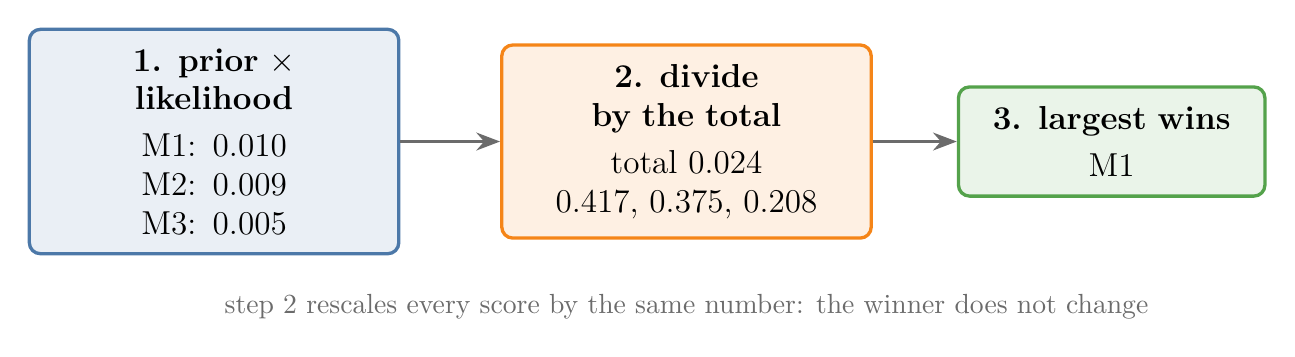
\begin{tikzpicture}[every node/.append style={font=\sffamily\large}]
  \node[box=cblue, text width=4.2cm] (s1) at (0,0) {\textbf{1. prior $\times$ likelihood}\\[3pt] M1: 0.010\\ M2: 0.009\\ M3: 0.005};
  \node[box=corange, text width=4.2cm] (s2) at (6,0) {\textbf{2. divide by the total}\\[3pt] total 0.024\\ 0.417, 0.375, 0.208};
  \node[box=cgreen, text width=3.4cm] (s3) at (11.4,0) {\textbf{3. largest wins}\\[3pt] M1};
  \draw[arrow] (s1) -- (s2);
  \draw[arrow] (s2) -- (s3);
  \node[note, font=\sffamily] at (6,-2.1) {step 2 rescales every score by the same number: the winner does not change};
\end{tikzpicture}
\end{document}
